\section{Commercial and Business Assessment}

% \subsection{Condition of Commercial Structures}

% \noindent \hl{[redo assessor map with commerical-listed parcels]}

\subsection{Business Establishments}

\noindent Over the last five years, the number of business establishments in Knox County has changed very little. \textbf{Figure~\ref{fig:bizEstablishments}} shows that the total number of businesses has decreased by just two during this time. All of the business loss is driven by fewer government establishments, while the number of private sector businesses has increased.

\begin{figure}[H]
\centering
\begin{framed}
    \caption{Business Establishments in Knox County, Nebraska}
    \label{fig:bizEstablishments}
    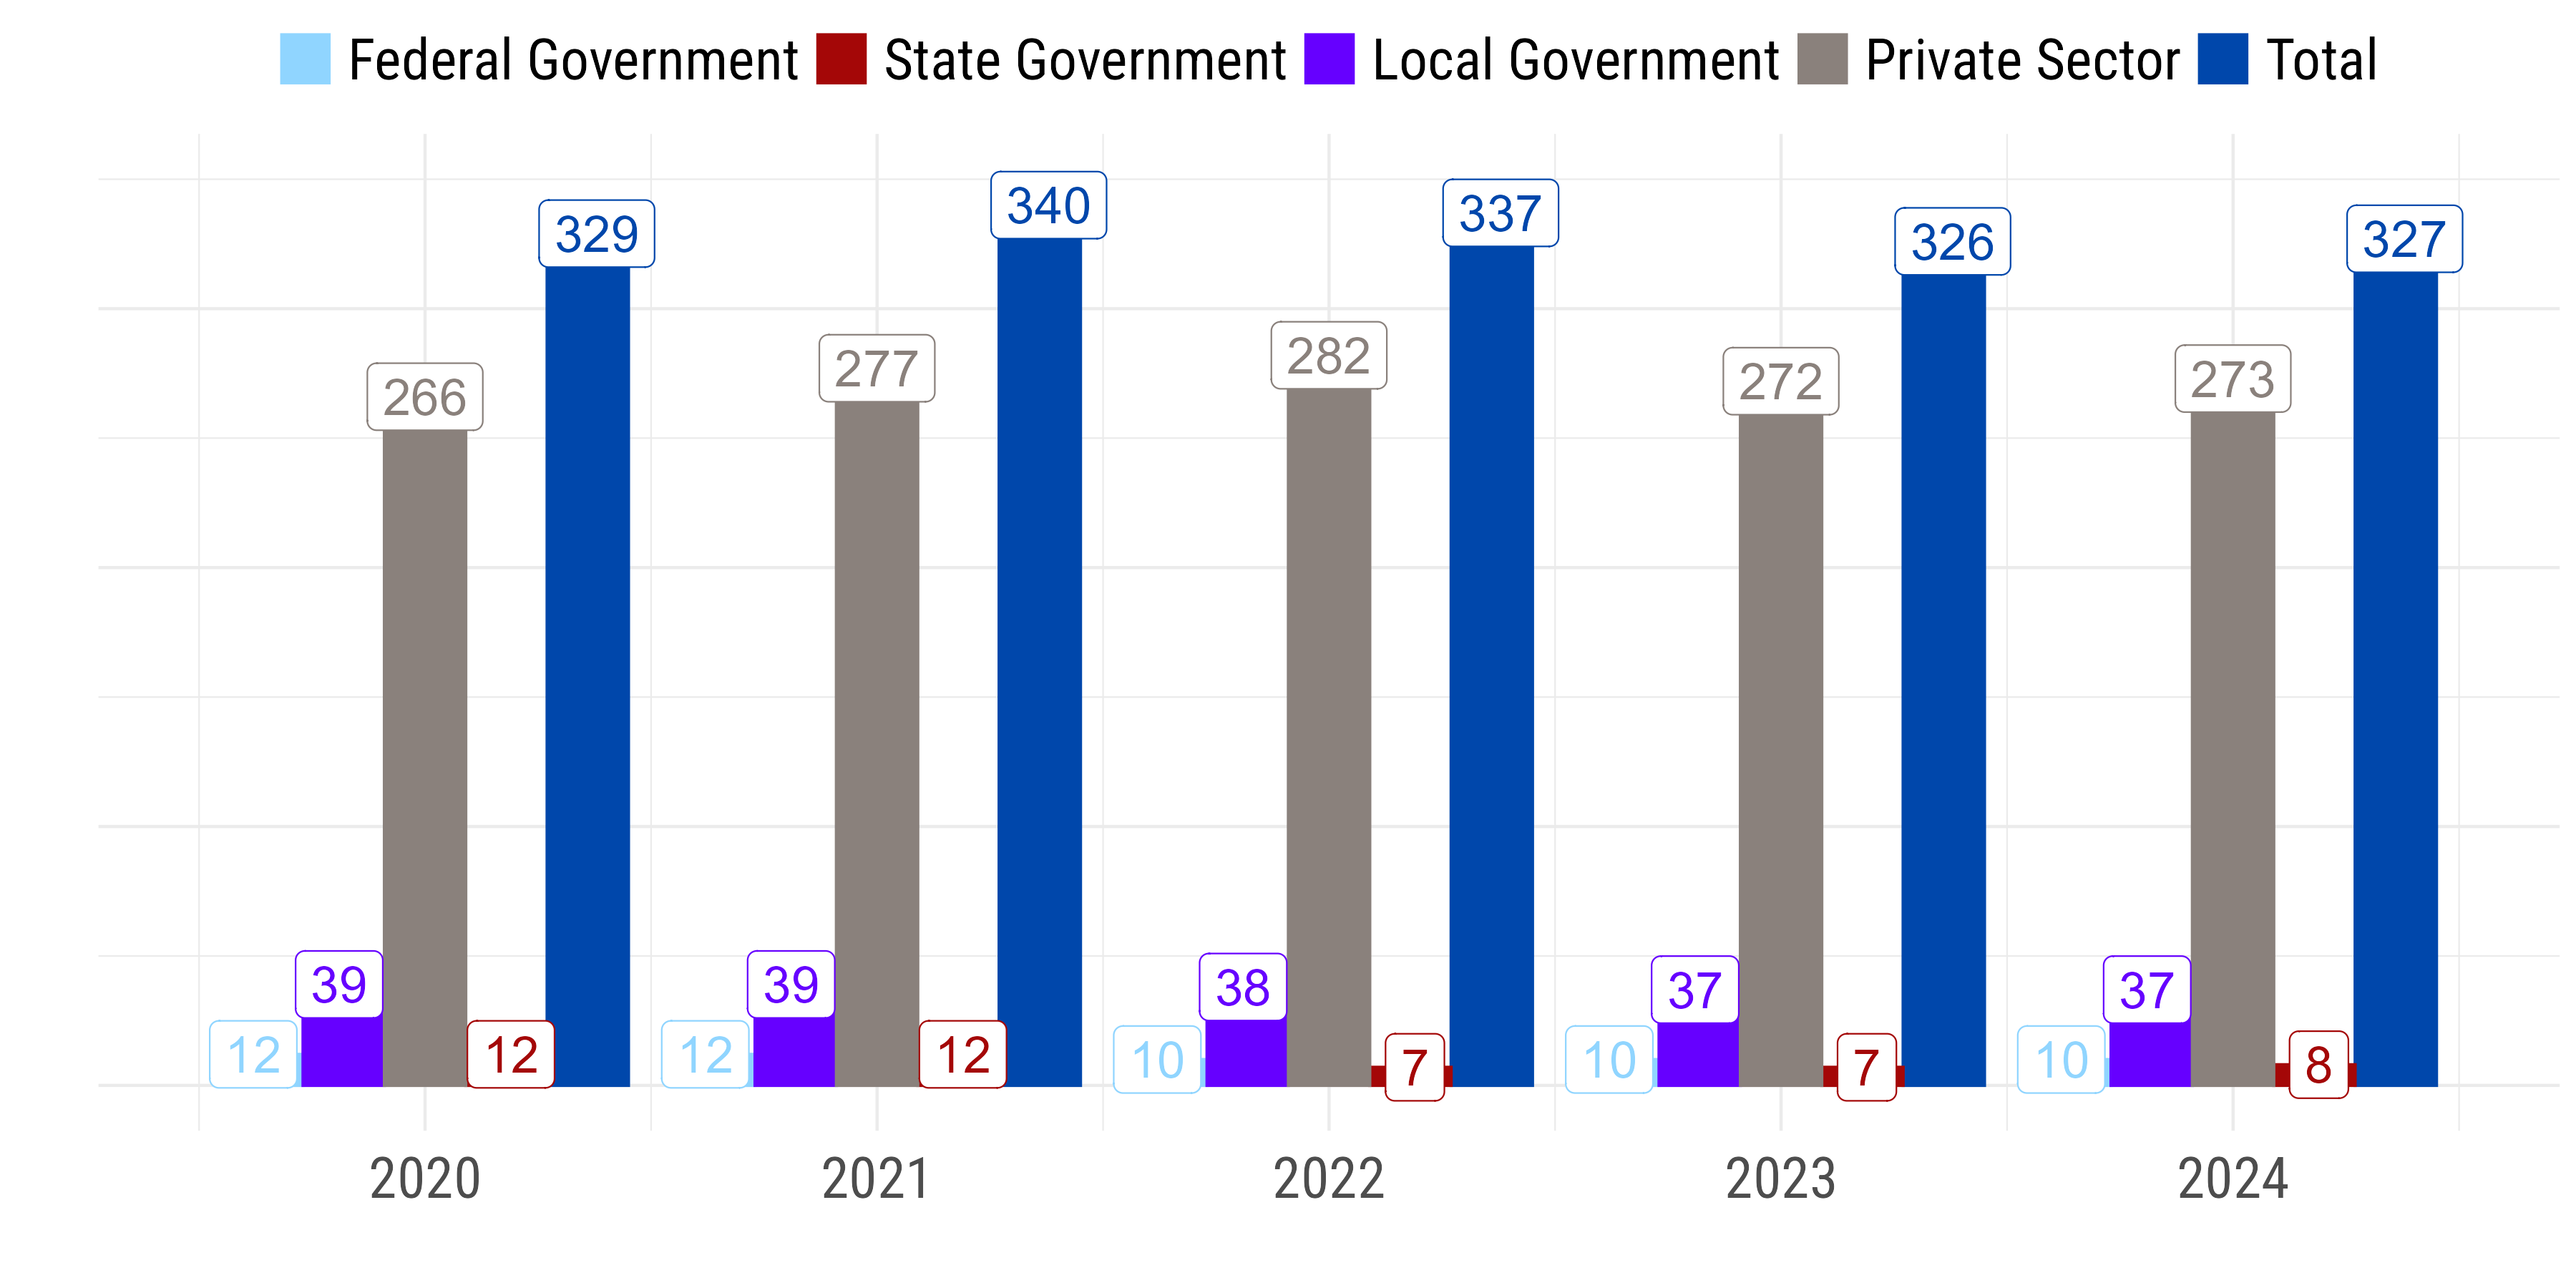
\includegraphics[width=\linewidth]{figures/knox_county_employers.png}
    \rule[-5pt]{\linewidth}{0.4pt}
    \floatnote{Data come from the \href{https://www.bls.gov/cew/}{Bureau of Labor Statistics Quarterly Census of Employment and Wages}.}
\end{framed}
\end{figure}


% \subsubsection{Auto Services and Freight Carriers}
% \subsubsection{Banking and Insurance}
% \subsubsection{Churches and Civic Organizations}
% \subsubsection{Communications}
% \subsubsection{Construction, Electricity, and Welding}
% \subsubsection{Grocery}
% \subsubsection{Hair Salon and Barbershop}
% \subsubsection{Lodging}
% \subsubsection{Medical and Pharmaceutical Services}
% \subsubsection{Nursing and Assisted Living}
% \subsubsection{Professional Services}
% \subsubsection{Residential Services}
% \subsubsection{Restaurants, Liquor, and Hospitality}
% \subsubsection{Retail}

\pagebreak
\subsection{Labor and Wages}

\noindent Similarly, most of the employees in Knox County are employed by local governments or private firms. \textbf{Figure~\ref{fig:employment}} shows that the county has experienced minor job growth since 2020. However, most of these gains were seen in government jobs, while private-sector employment fell by about two percent in that time.

\begin{figure}[H]
\centering
\begin{framed}
    \caption{Employment in Knox County, Nebraska}
    \label{fig:employment}
    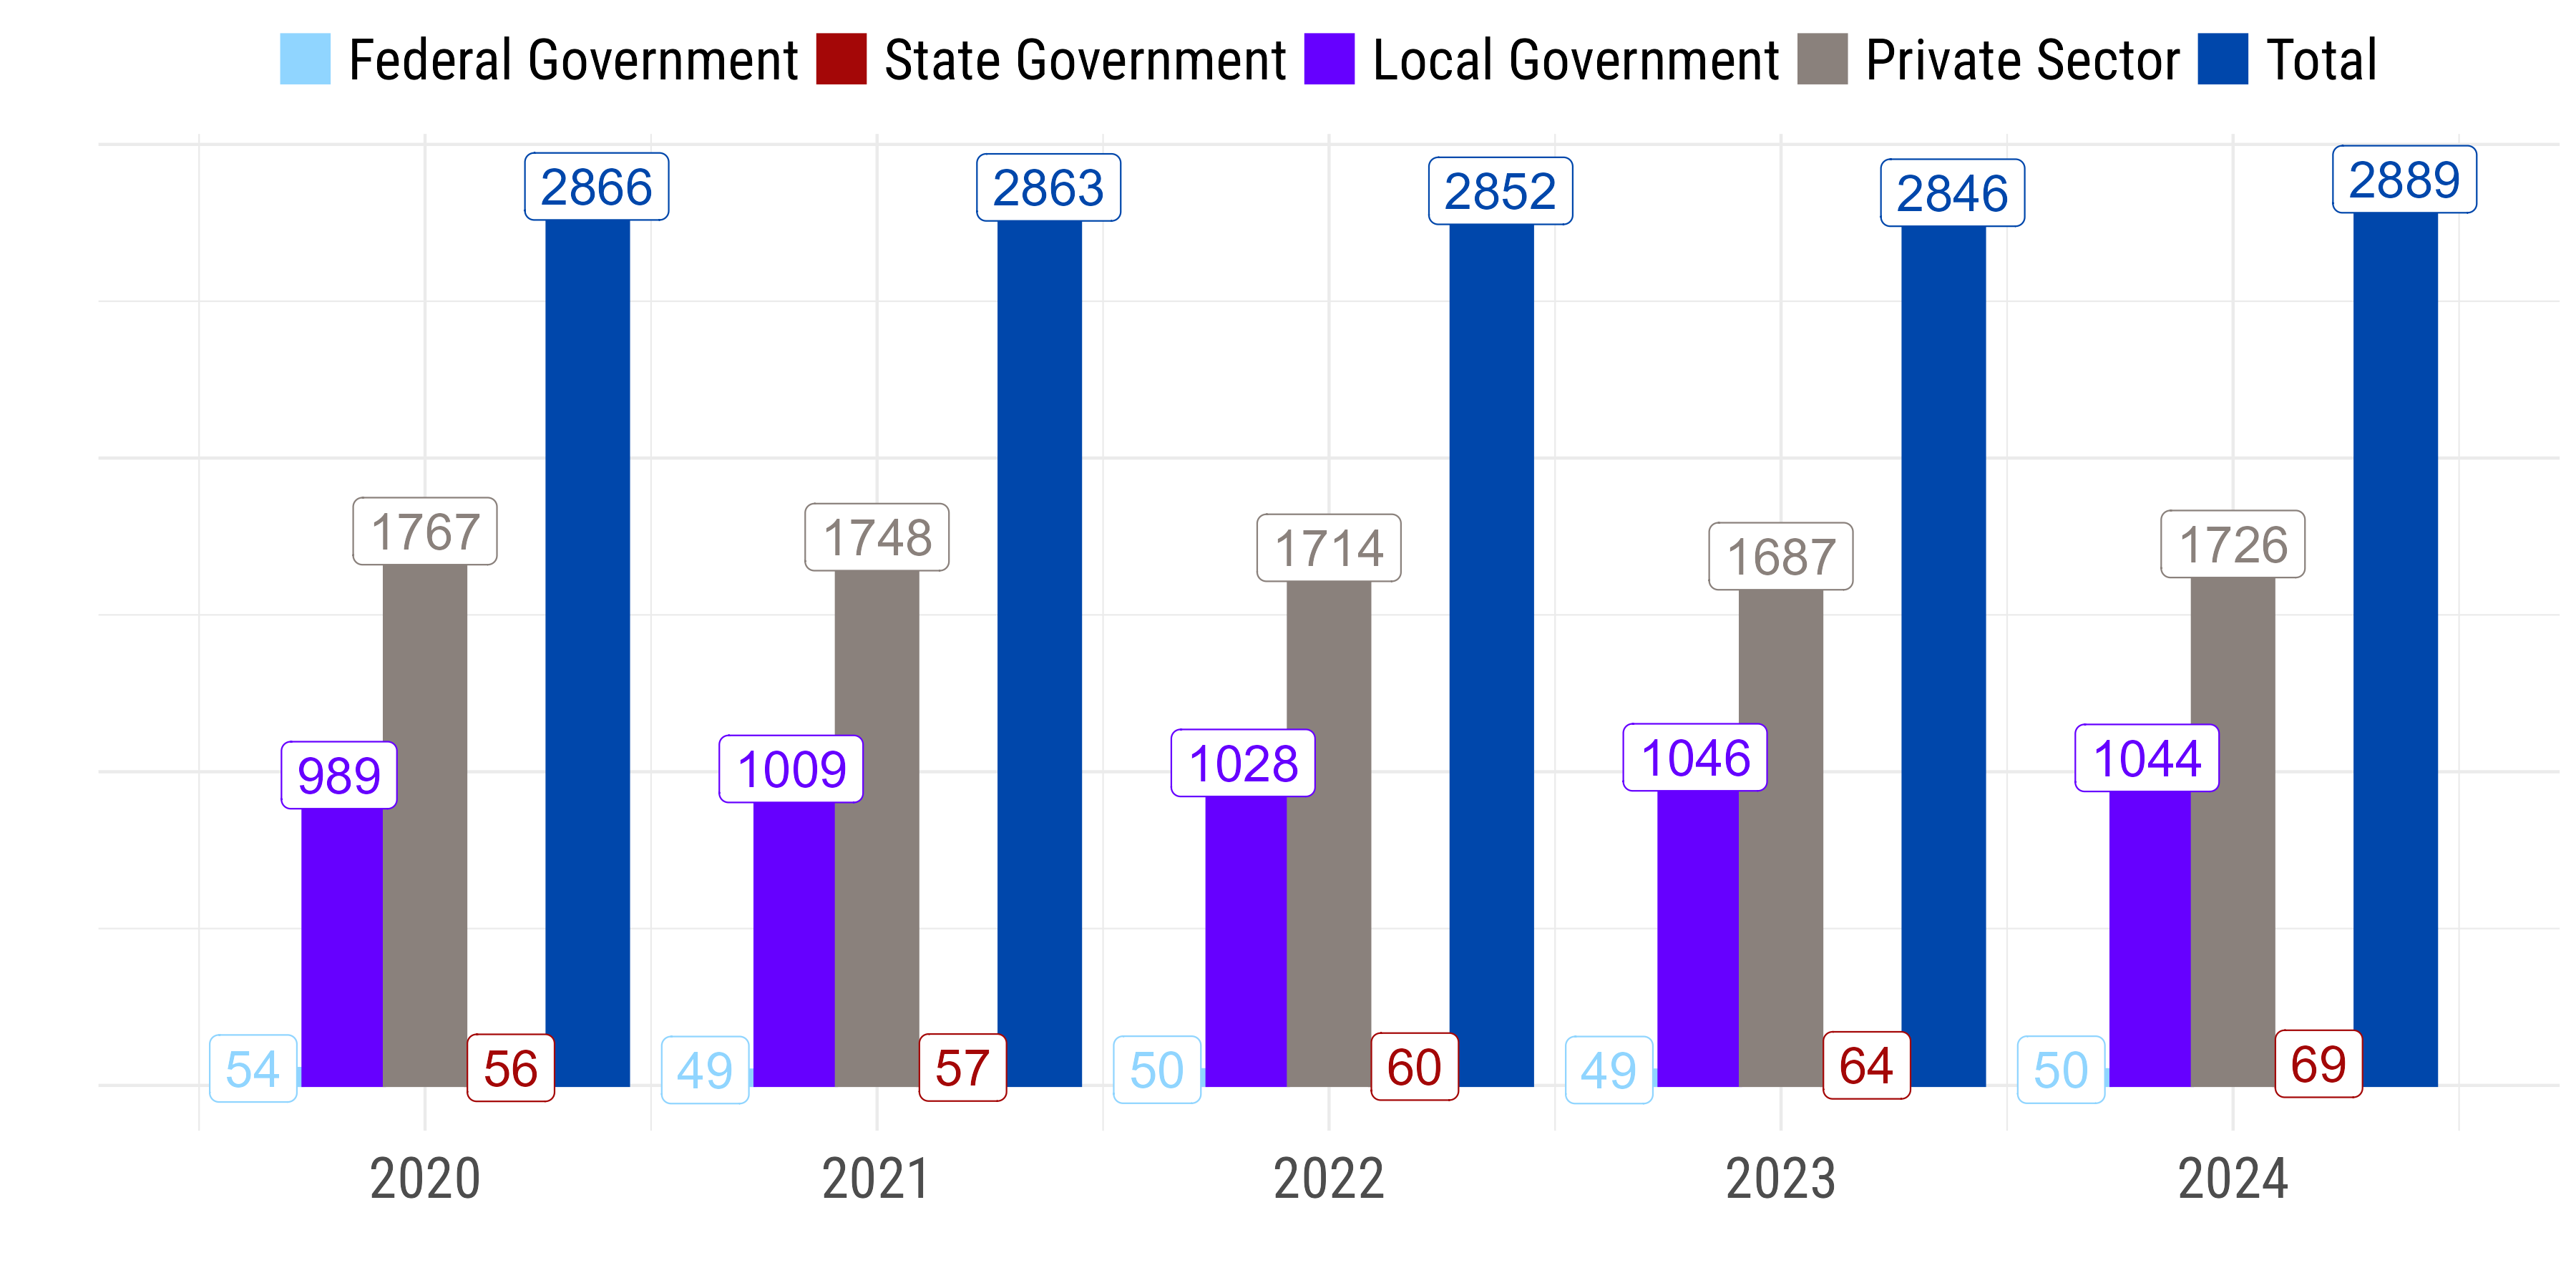
\includegraphics[width=\linewidth]{figures/employment.png}
    \rule[-5pt]{\linewidth}{0.4pt}
    \floatnote{Data come from the \href{https://www.bls.gov/cew/}{Bureau of Labor Statistics Quarterly Census of Employment and Wages}.}
\end{framed}
\end{figure}

\pagebreak

\noindent Across the board, real wages in Knox County increaed over the span of 2020 to 2023. However, these gains were largely erased in 2024 (\textbf{Figure~\ref{fig:wages}}). More time is needed to tell whether wage decreases are a blip or the beginning of a broader downward trend.

\begin{figure}[H]
\centering
\begin{framed}
    \caption{Real Wages in Knox County, Nebraska}
    \label{fig:wages}
    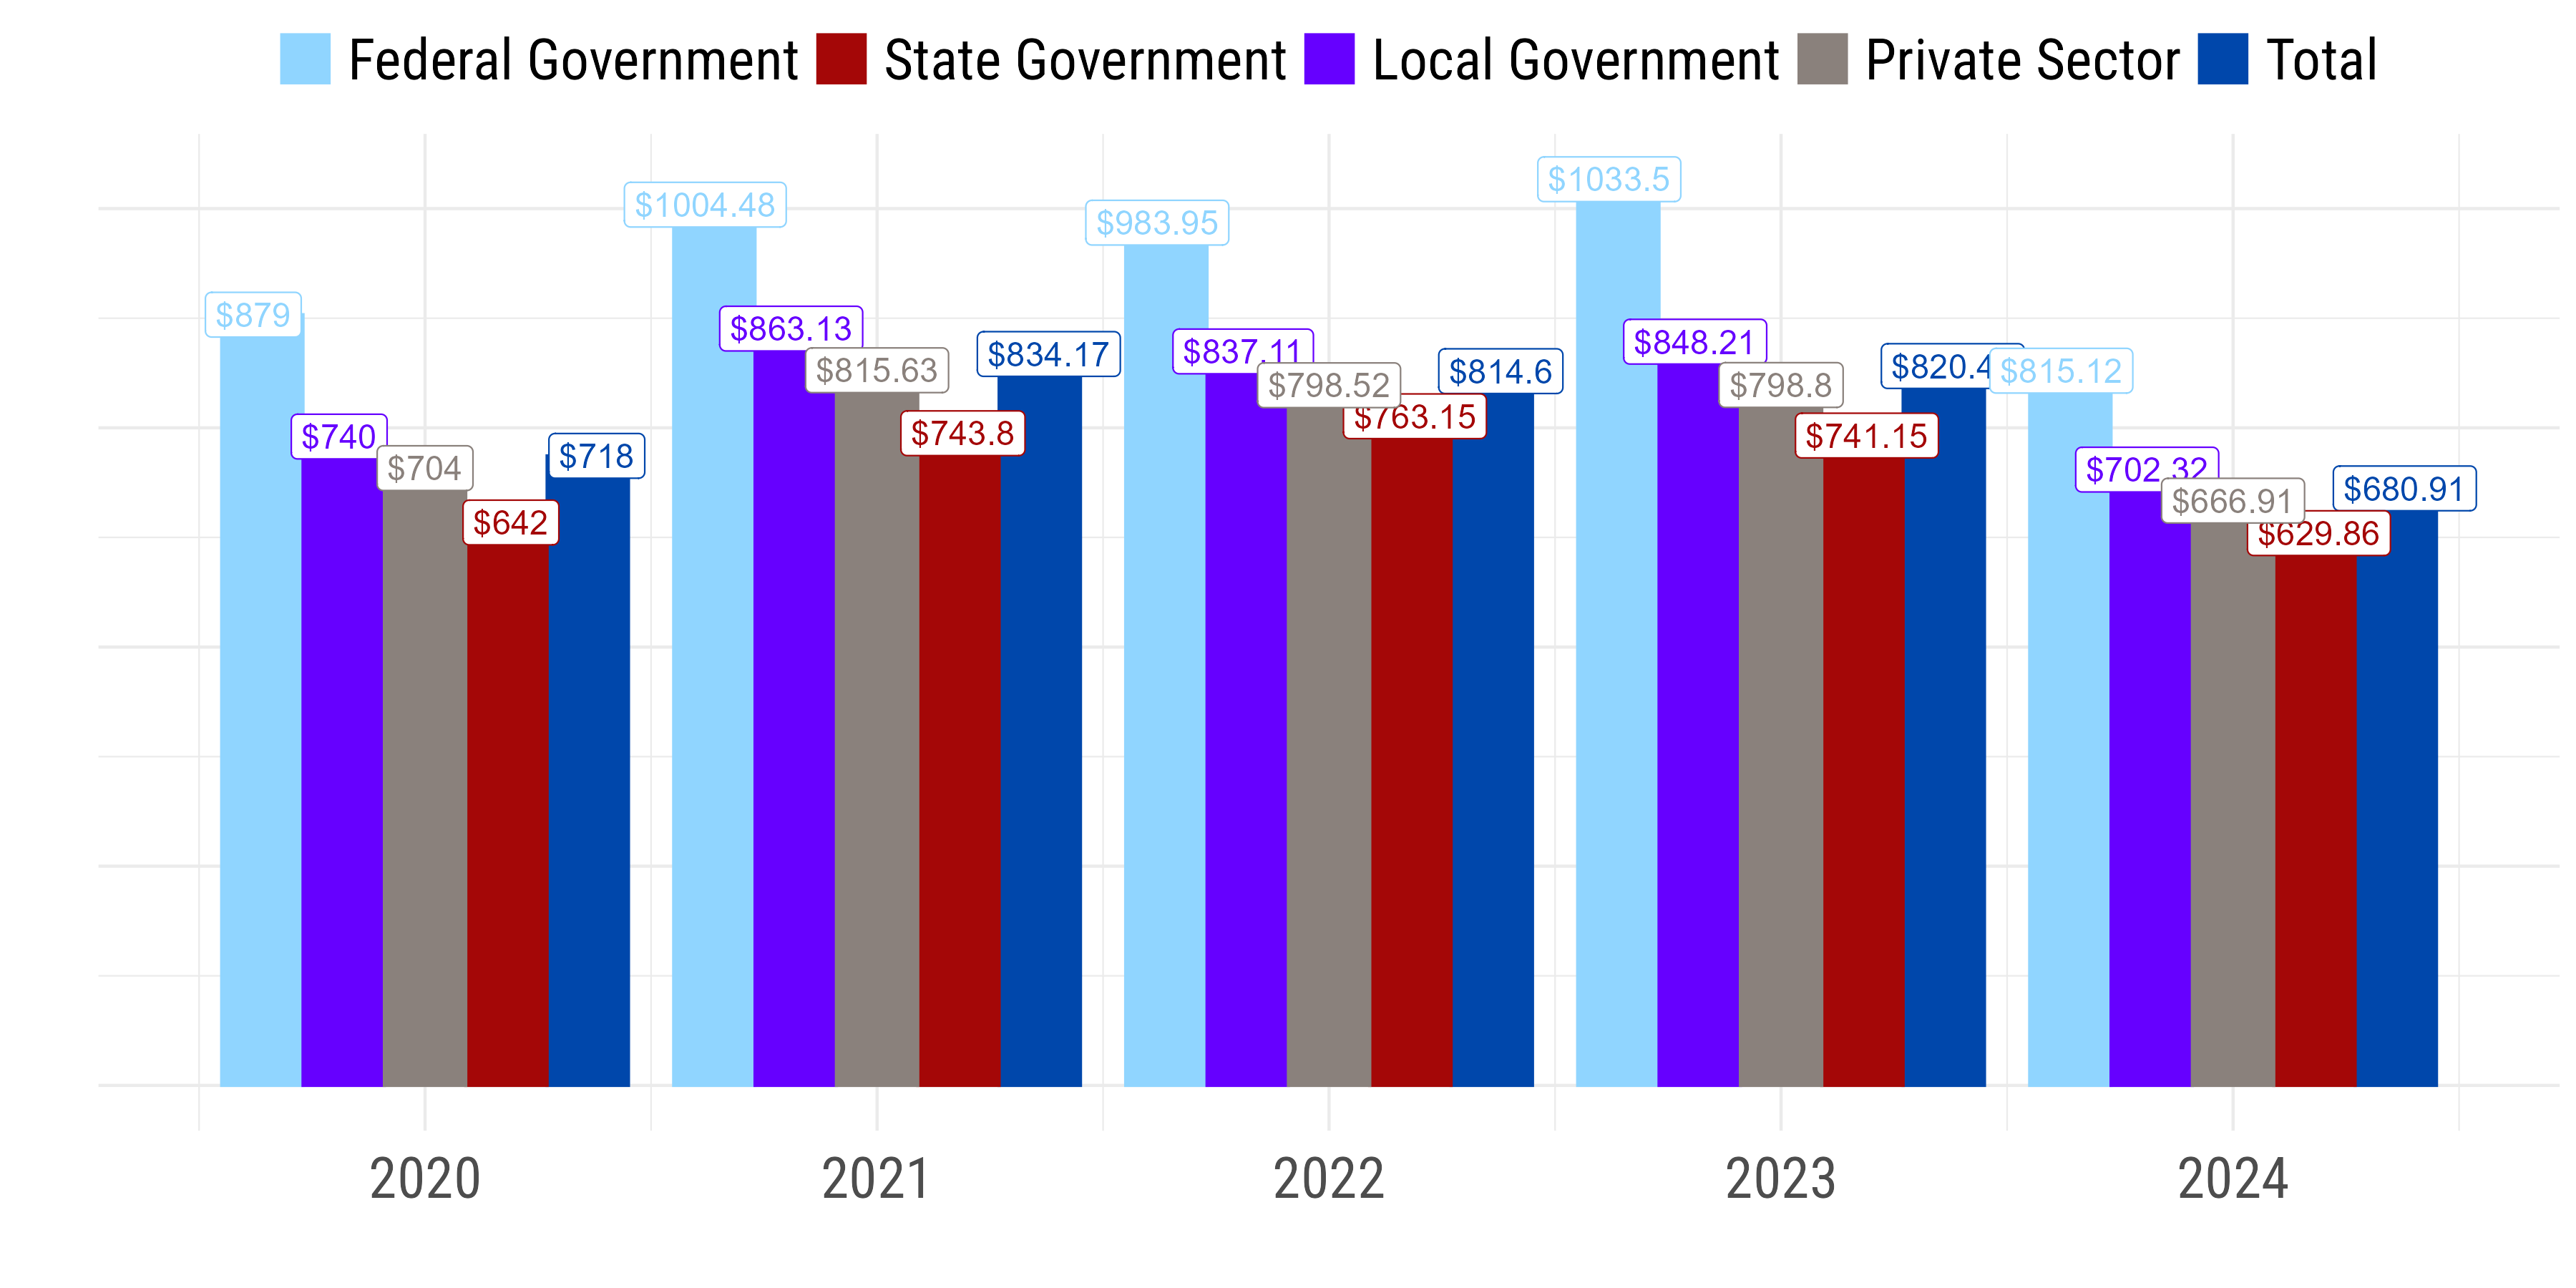
\includegraphics[width=\linewidth]{figures/avg_weekly_wage.png}
    \rule[-5pt]{\linewidth}{0.4pt}
    \floatnote{Data come from the \href{https://www.bls.gov/cew/}{Bureau of Labor Statistics Quarterly Census of Employment and Wages}. Units are in 2024-adjusted real dollars.}
\end{framed}
\end{figure}

\subsection{Economic Activity}

\noindent Overall economic activity in Bloomfield and other comparable cities has varied over the last decade. \textbf{Figure~\ref{fig:netTaxableSales}} shows how, adjusting for inflation, the cumulative volume of taxable sales in Bloomfield has increased by about nine percent. In nearby Creighton, it has decreased by about eight percent. And in Crofton, excluding an outlier year in 2014, the volume of net taxable sales has decreased by about two percent.

\begin{figure}[H]
\centering
\begin{framed}
    \caption{Net Taxable Sales in Knox County, Nebraska}
    \label{fig:netTaxableSales}
    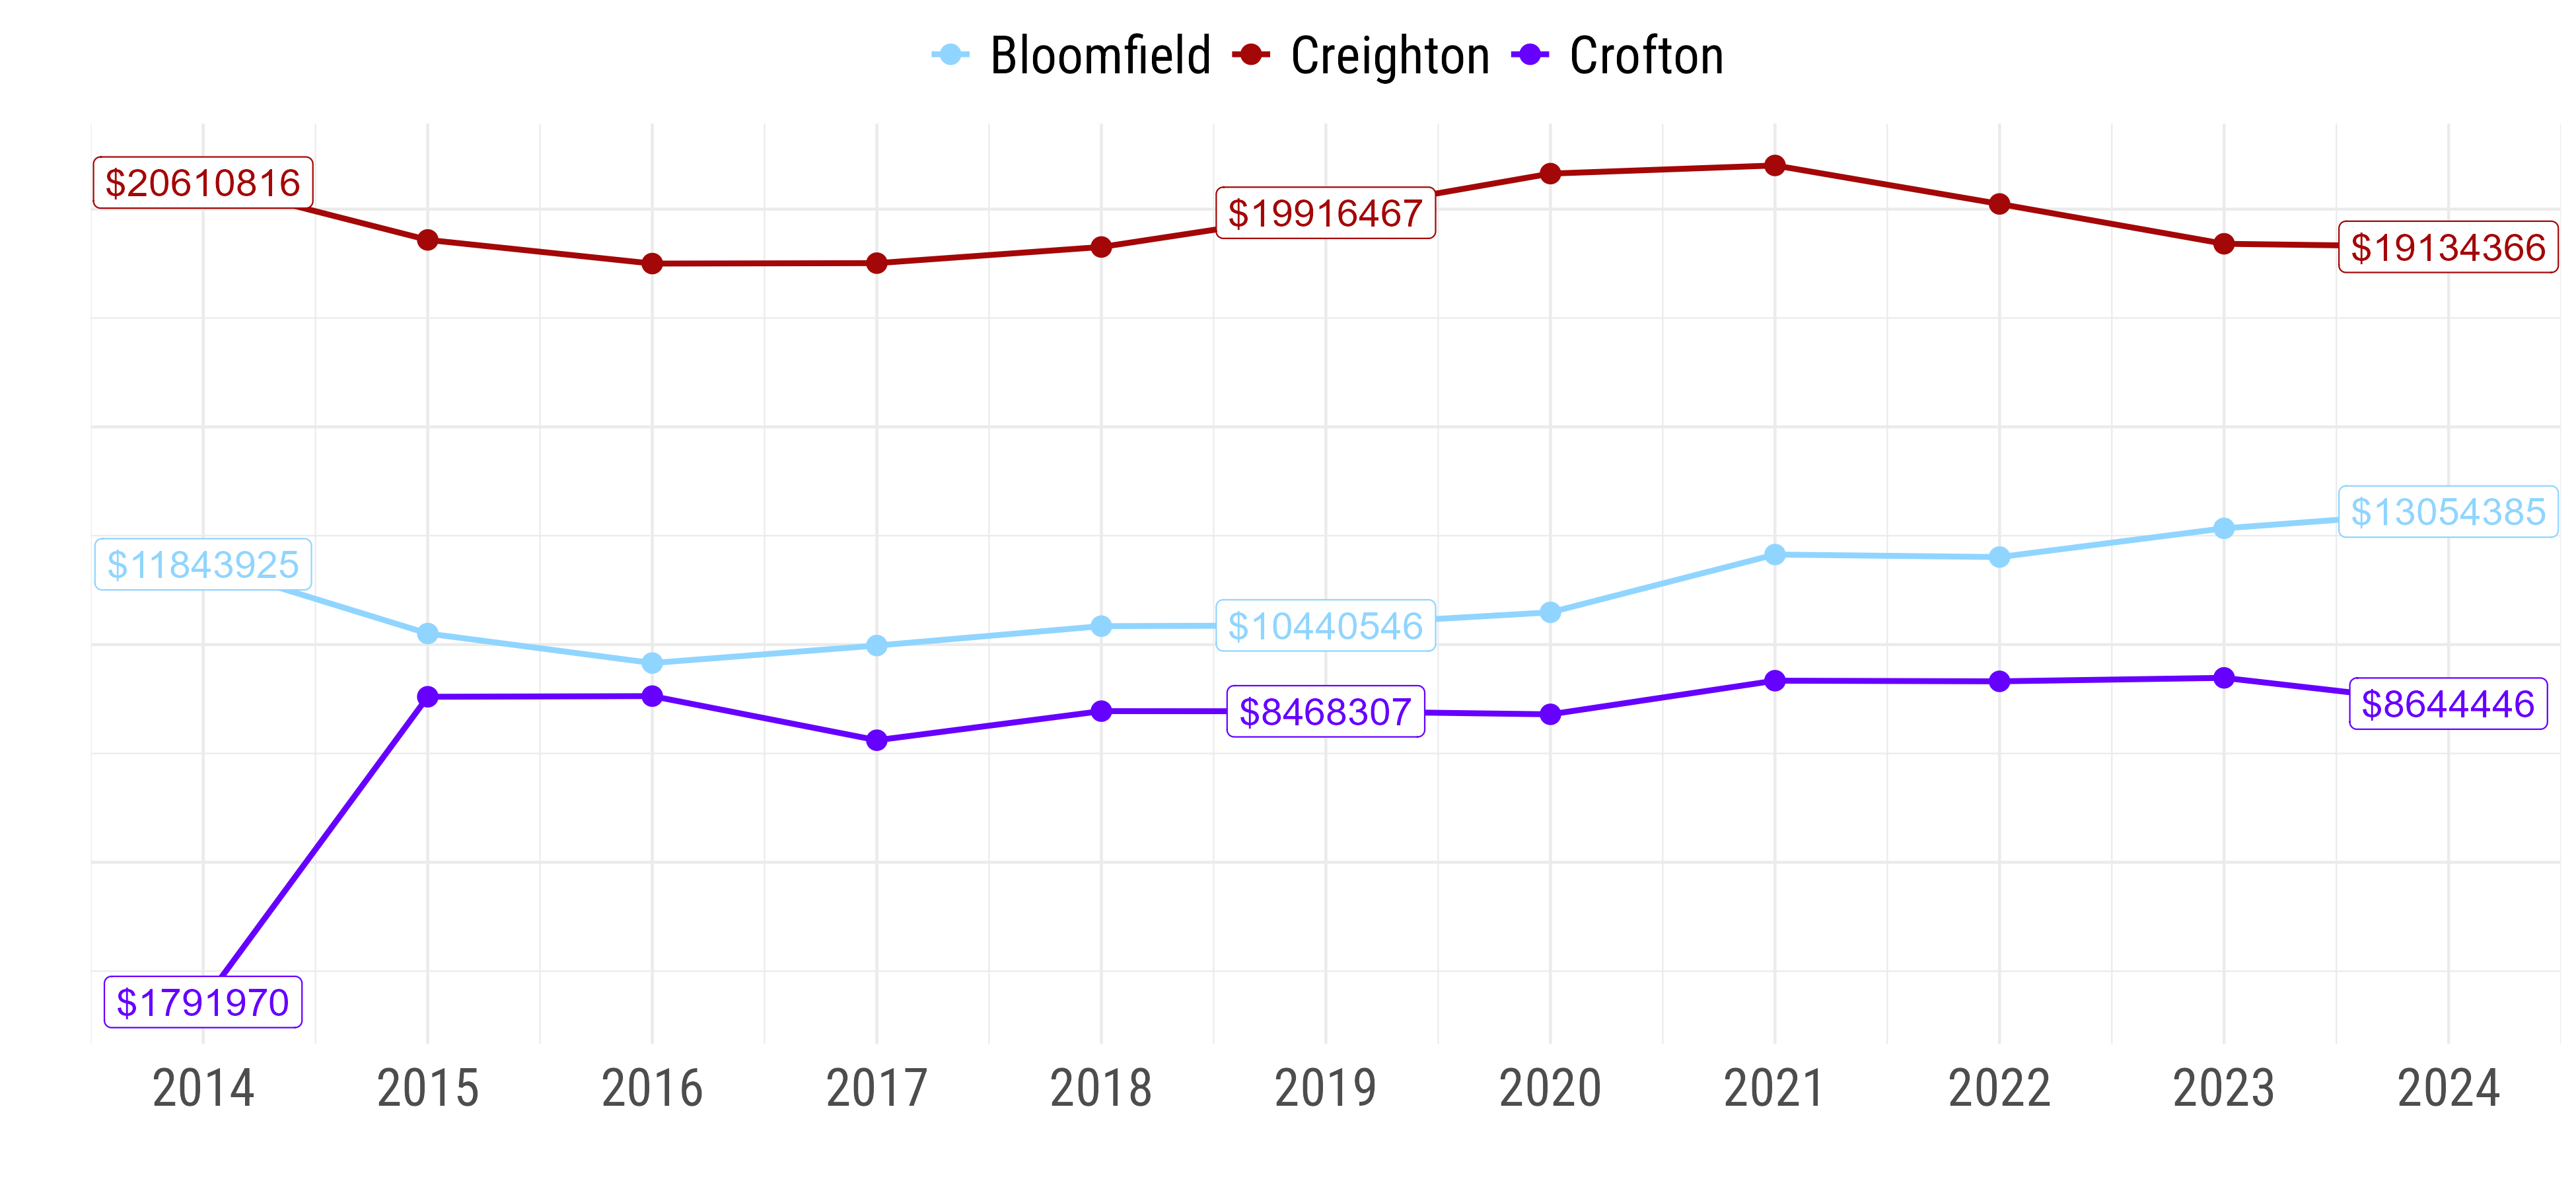
\includegraphics[width=\linewidth]{figures/net_taxable_sales.png}
    \rule[-5pt]{\linewidth}{0.4pt}
    \floatnote{Data come from the \href{https://revenue.nebraska.gov/research/statistics/sales-tax-data}{Nebraska Department of Revenue}. Units are in 2024-adjusted real dollars.}
\end{framed}
\end{figure}

\noindent Furthermore, agriculture is an integral part of Bloomfield's (and Knox County generally) economy. \textbf{Figure~\ref{fig:agProduction}} shows how agricultural production, establishments, and employment have evolved over the past century. Livestock and crop yields generally peaked in the early 1990s but have slowly declined since. Employment in the sector is down since 2000. Most strikingly, the number of independent farms in Knox County has steadily decreased, likely due to practices of corporate consolidation.

\begin{figure}[H]
\centering
\begin{framed}
    \caption{Agricultural Production and Labor in Knox County, Nebraska}
    \label{fig:agProduction}
    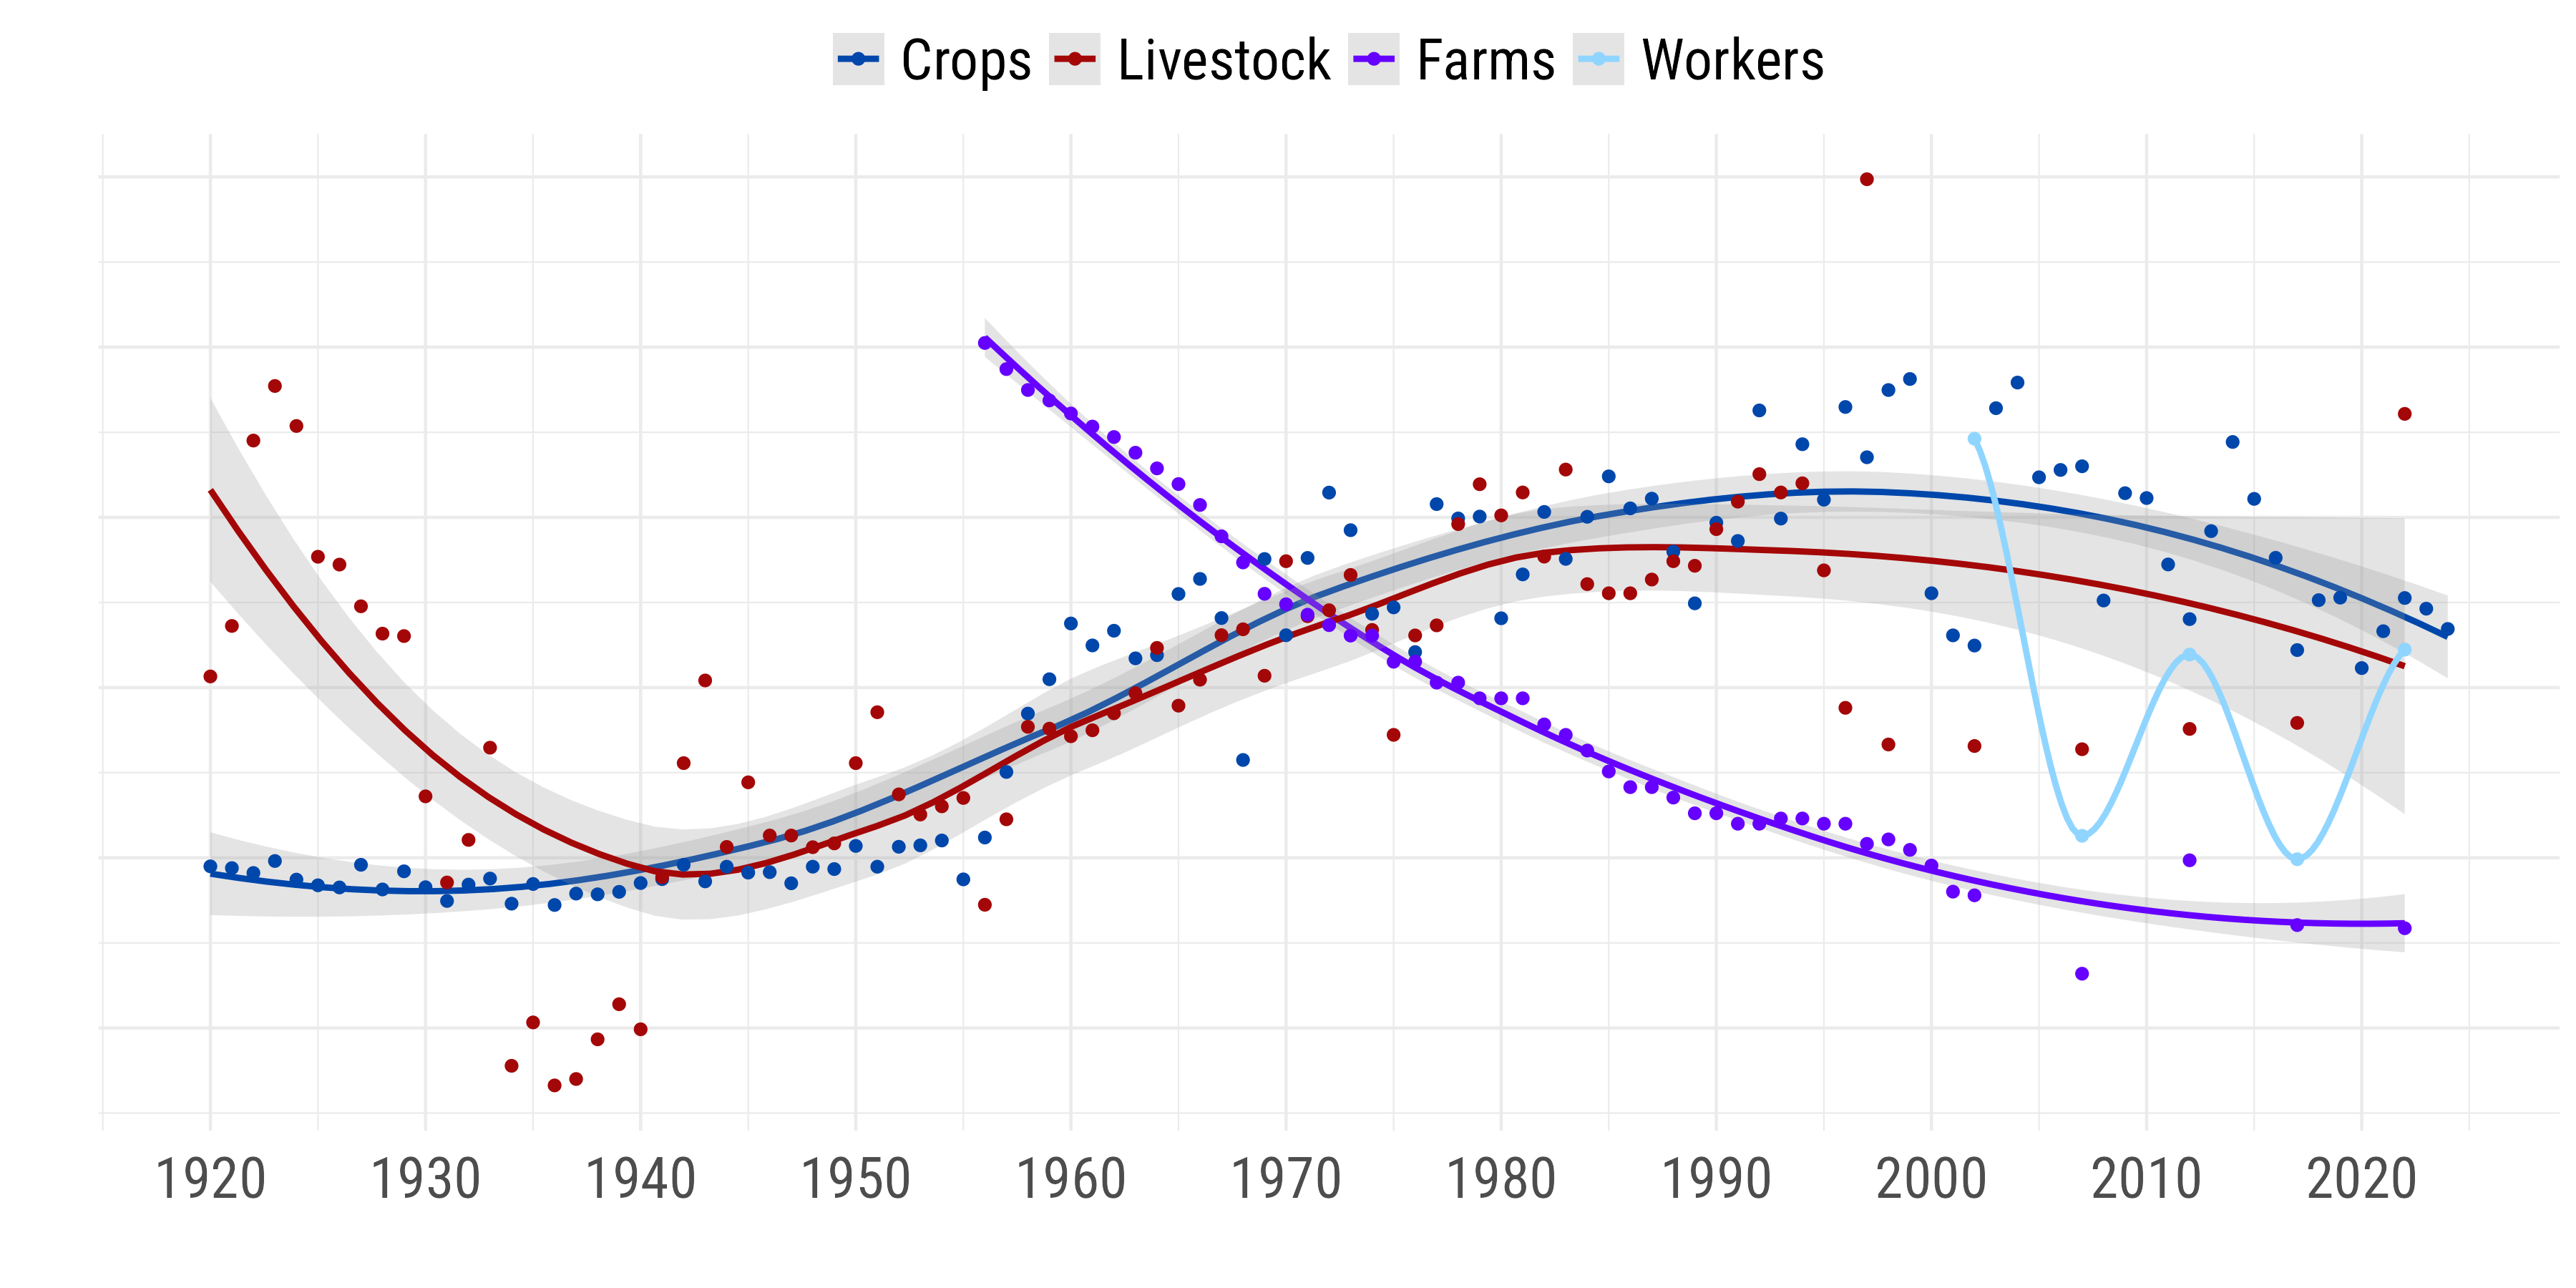
\includegraphics[width=\linewidth]{figures/ag_production.png}
    \rule[-5pt]{\linewidth}{0.4pt}
    \floatnote{Data come from the \href{https://www.nass.usda.gov/AgCensus/}{United States Department of Agriculture National Agricultural Statistics Service}. All units are standardized to reflect relative, not absolute, growth and decline.}
\end{framed}
\end{figure}

\pagebreak
\subsection*{Key Takeaways}